\section{Further discussion on the positional-semantic transition} \label{2506:app:further-positional-demantic}
% \subsection{Adding the value matrix}
% So far we have considered the case where the value matrix is the identity matrix
% \(
%     V = I_L,
% \)
% because we are not interested in a new representation of the input, but rather in a low dimensional label. In this subesction we show that fo the 



\subsection{SIE of model \eqref{2506:eq:positional-semantic-label}}
Definition~\ref{2506:def:sie} of the sequence information exponent does not apply directly to the model \eqref{2506:eq:positional-semantic-label} because the model has a non-scalar output. However, we can still extend the concept of SIE to this case by looking at the update rule of sufficient statistics around initialization.

The population loss function is given by
\begin{equation}\begin{split}
    R(e,m) &= \mathbb{E}_{\vec{z},\vec{z}_\star \sim \mathcal{P}(e,m)} \Biggl[\Biggl\lVert
        (1-\omega) \SoftMax\left(\vec{z}_\star \vec{z}_\star^\top \right) + \omega \SoftMax\left[\begin{pmatrix}
        a^2 & -a^2 \\
        -a^2 & a^2 \\
    \end{pmatrix}\right] \\
    &\qquad\qquad {}- \SoftMax\left(\vec{z} \vec{z}^\top \right)
    \Biggr\rVert_F\Biggr] \\
    &= \mathbb{E}_{\vec{z},\vec{z}_\star \sim \mathcal{P}(e,m)} \left[\mathcal{L}(\vec{z},\vec{z}_\star)\right]
\end{split}\end{equation}
with
\begin{equation}
    \mathcal{P}(e,m) \equiv \mathcal{N}\left(
        \begin{pmatrix} 0\\ 0\\ e\\ -e \end{pmatrix},
        \begin{pmatrix}
            1 & 0 & m & 0 \\
            0 & 1 & 0 & m \\
            m & 0 & 1 & 0 \\
            0 & m & 0 & 1
        \end{pmatrix}
    \right).
\end{equation}
Using parity arguments, we can easily show that the gradient of the population loss is 0 at the initialization point \((e,m) = (0,0)\). Let \(p(\vec{z}_\star,\vec{z};e,m)\) be the probability density function associated with the distribution \(\mathcal{P}(e,m)\). Then the gradient at initialization is
\begin{equation}
    \left.\nabla_{(e,m)} R(e,m)\right|_{e=m=0} = \mathbb{E}_{\vec{z},\vec{z}_\star\sim\mathcal{P}(e,m)}\left[
        \frac{\nabla_{(e,m)}p(\vec{z}_\star,\vec{z};e,m)}{p(\vec{z}_\star,\vec{z};0,0)}
        \mathcal{L}(\vec{z},\vec{z}_\star)
    \right] 
\end{equation}
\(\mathcal{L}(\vec{z}_\star,\vec{z})\) is an even function of \((\vec{z}_\star,\vec{z})\), while the gradient of the probability density function is an odd function of \((\vec{z}_\star,\vec{z})\). Therefore, the product is an odd function of \((\vec{z}_\star,\vec{z})\) and the expectation is 0.
\begin{equation}
    \left.\nabla_{(e,m)} R(e,m)\right|_{e=m=0} = (0,0).
\end{equation}
We can use the same computation technique to compute the Hessian of the population loss at initialization. This time the parity arguments does not apply, and we can show numerically that the Hessian is non-null
\begin{equation}
    \left.\frac{\partial^2 R}{\partial e^2}\right|_{e=m=0},
    \left.\frac{\partial^2 R}{\partial m^2}\right|_{e=m=0},
    \left.\frac{\partial^2 R}{\partial e \partial m}\right|_{e=m=0} \neq 0.
\end{equation}

\paragraph{The information exponent}
 We can also compute the \textit{information exponent} by looking at what rate \(m\) grows around initialization. We use \emph{spherical gradient descent} beacuse we assumed the norm of the vector \(\vec w\) to be costant (as Ben Arous also does in his paper on Information Exponent):

 The update rule of \(\vec w\) is
 \[
    \vec{w}^{\tau+1} = \frac{\vec{w}^\tau - \gamma \nabla_{\vec{w}}\mathcal{L}}{\norm{\vec{w}^\tau - \gamma \nabla_{\vec{w}}\mathcal{L}}}_2\sqrt{d},
 \]
 multiplying both sides by \(\sfrac{\vec{w}_\star}{d}\) we get
  \[
    m^{\tau+1} = \frac{m^\tau - \gamma \frac{\vec{w}_\star\cdot\nabla_{\vec{w}}\mathcal{L}}{d}}{\norm{\vec{w}^\tau - \gamma \nabla_{\vec{w}}\mathcal{L}}_2}\sqrt{d}.
 \]
We can assume to be in the \emph{gradient flow regime}, where the learning rate \(\gamma \ll 1\)
\[
   \norm{\vec{w} - \gamma \nabla_{\vec{w}}\mathcal{L}}_2 =
    \sqrt{\norm{w}^2-2\gamma \vec{w}\cdot\nabla_w\mathcal{L} + \gamma^2\norm{\nabla_w\mathcal{L}}^2}
        \approx \sqrt{d} \sqrt{1-2\gamma \frac{\vec{w}\cdot\nabla_w\mathcal{L}}{d}},
\]
that finally lead us to
\begin{equation} \label{2506:eq:m-update-normalized-gradient}
    m^{\tau+1} = \left(m^\tau - \gamma \frac{\vec{w}_\star\cdot\nabla_{\vec{w}}\mathcal{L}}{d}\right)\left(1+\gamma \frac{\vec{w}\cdot\nabla_w\mathcal{L}}{d}\right)
    \approx m^\tau - \gamma \frac{\vec{w}_\star\cdot\nabla_{\vec{w}}\mathcal{L}}{d} + \gamma \frac{\vec{w}\cdot\nabla_w\mathcal{L}}{d},
\end{equation}
where in the last step we used again the small learning rate limit.
 
 Now we can use the chain rule for getting the gradient in terms of the derivatives we already have
 \[
    \nabla_w \mathcal{L} = \frac{\partial \mathcal{L}}{\partial m}\cdot \nabla_{\vec{w}}m + \frac{\partial \mathcal{L}}{\partial e}\cdot \nabla_{\vec{w}}e =
    \frac{\partial \mathcal{L}}{\partial m}\cdot \frac{\vec{w}_\star}{d} + \frac{\partial \mathcal{L}}{\partial e}\cdot \frac{\vec p}{\sqrt{d}}
 \]
 We can rearrange the equation above as
 \[\begin{split}
    \frac{m^{\tau+1} - m^\tau}{\sfrac{\gamma}{d}} =& -\vec{w}_\star \cdot \left(\frac{\partial \mathcal{L}}{\partial m}\cdot \frac{\vec{w}_\star}{d} + \frac{\partial \mathcal{L}}{\partial e}\cdot \frac{\vec p}{\sqrt{d}}\right) + \vec{w} \cdot \left(\frac{\partial \mathcal{L}}{\partial m}\cdot \frac{\vec{w}_\star}{d} + \frac{\partial \mathcal{L}}{\partial e}\cdot \frac{\vec p}{\sqrt{d}}\right) \\=& -\frac{\partial \mathcal{L}}{\partial m} + m\frac{\partial \mathcal{L}}{\partial m} + e\frac{\partial \mathcal{L}}{\partial e}
 \end{split}\]
 where we used the fact \(\vec p \cdot \vec{w}_\star \approx 0\) in high dimension (as already assumed above), and \(\norm{\vec{w}_\star}=d\).

 We are interested in what is happening at initialization, therefore all the derivatives should be evaluated around \((e,m)=0\). We already know that \(\left.\nabla_{e,m}\mathcal{L}\right|_{e=m=0}=0,\) so we expand the at the next order in \(m\)
\[
 \frac{m^{\tau+1} - m^\tau}{\sfrac{\gamma}{d}} =
    -m\left.\frac{\partial^2 \mathcal{L}}{\partial m^2}\right|_{m,e=0} + 2 me \left.\frac{\partial^2 \mathcal{L}}{\partial m\partial e}\right|_{m,e=0}.
 \]
 We can repeat the same derivation for finding the analogous equation for \(e\):
 \[
 \frac{e^{\tau+1} - e^\tau}{\sfrac{\gamma}{d}} =
    -e\left.\frac{\partial^2 \mathcal{L}}{\partial e^2}\right|_{m,e=0} + 2 me \left.\frac{\partial^2 \mathcal{L}}{\partial m\partial e}\right|_{m,e=0}.
 \]
 Since the hessian of he loss has always a negative eigenvalue, both these equations need \(\tau = O(d\log d)\) to escape a neighborhood of initialization, leading to \(\text{IE}=2\).

\subsection{Numerical experiments on the transition}
In this Appendix we would like to provide more details on the phase diagram of Figure~\ref{2506:fig:phase-diagram-postional-semantic}. 

In Figure \ref{2506:fig:app:trajectories-d100-positional-semantic} we reproduce Figure~\ref{2506:fig:positional-semantic-trajectories-a1} for \(d=100\), clarifying the \emph{finite size} effects we claimed in the main text. Smaller values of \(d\) lead to a more smooth transition, since the grndient flow assumption is less valid. In the limit \(d\to\infty\) we expect to see a step function.
\begin{figure}
    \centering
    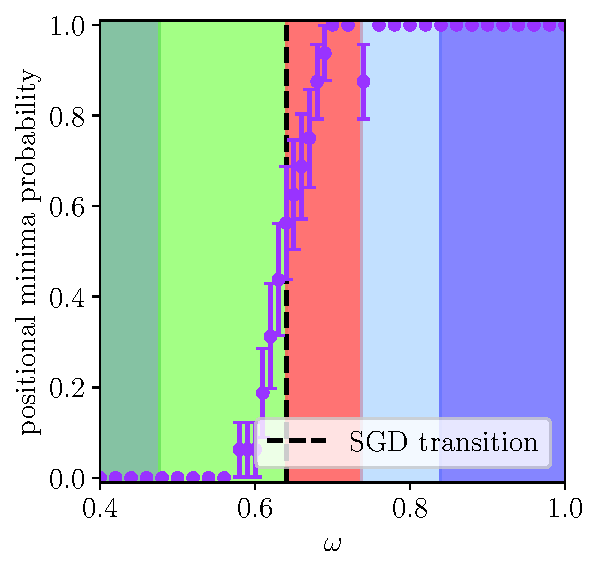
\includegraphics[width=0.4\textwidth]{figs/positional-semantic/trajecttories-probability-d100-a1}
    \caption{reproduction of Figure~\ref{2506:fig:positional-semantic-trajectories-a1} for \(d=100\). The transition is smoother than in the \(d=1000\). Averaged over 25 runs.
    }
    \label{2506:fig:app:trajectories-d100-positional-semantic}
\end{figure}

The yellow region in the phase diagram of Figure~\ref{2506:fig:phase-diagram-postional-semantic} is predicted to have a unique global semantic minima, while SGD is aligned with the positional direction at initialization. The resulting trajectories are shown in Figure~\ref{2506:fig:app:phase-diagram-yellow-region}: the dynamics moves towards the minima direction, get stuck in the local flat (but not critical) region around \((e,m)=(1,0)\), and then it moves towards the global minima. In this region the convergence is very slow.
\begin{figure}
    \centering
    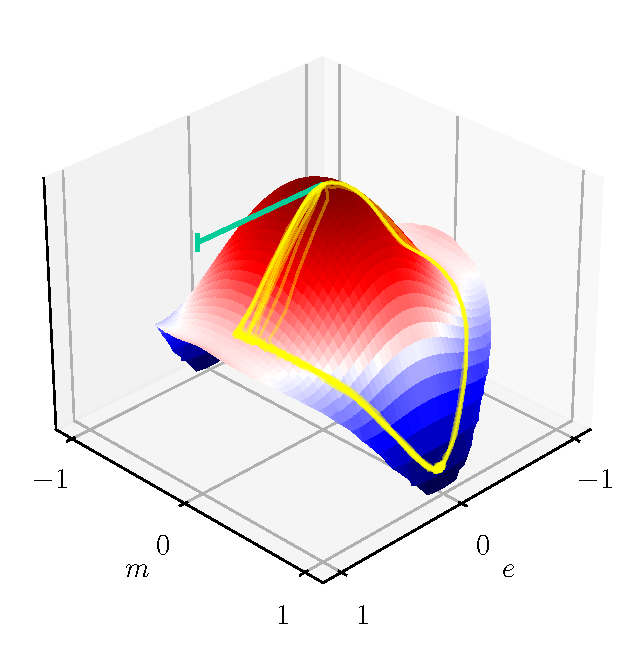
\includegraphics[width=0.4\textwidth]{figs/positional-semantic/loss_surface_omega0.95_a0.76}
    \caption{The loss surface in the yellow region of the phase diagram. The SGD trajectory is shown in yellow. The training moves towards the direction orthogonal to the one of global minima, ultimately slowing down the convergence.
    }
    \label{2506:fig:app:phase-diagram-yellow-region}
\end{figure}
The turning point of the dynamics is a bit misplaced because of the numerical errors given by the loss integration; details on this in Appendix~\ref{2506:app:numerical-details}.





\subsection{An alternative model without phase transition}
In order to highlight the peculiarity of the model \eqref{2506:eq:positional-semantic-label}, we present an example of a model that does not exhibit a phase transition between the positional and semantic regimes.
Let's assume that our target is a softmax attention matrix \emph{with} positional encoding
\[
y(X) = \SoftMax\left[(X+\sfrac{P_\star}{\sqrt{d}})\vec{w}_\star \vec{w}_\star^\top (X+\sfrac{P_\star}{\sqrt{d}})^\top\right]
\]
where 
\[
P_\star = \begin{pmatrix} +\vec{p}_\star \\ -\vec{p}_\star \end{pmatrix}, \qquad
\vec{w}_\star = \sqrt{1-\omega^2} \vec{w}_{s} + \omega \vec{p}_\star \sqrt{d}
\quad\text{with}\quad \vec{w}_{s} \bot \vec{p}_\star.
\]
\(\omega\) plays the same role as in the model \eqref{2506:eq:positional-semantic-label}, and we can set \(\omega=0\) to get the semantic model, or \(\omega=1\) to get the positional model. The difference is that in this case the positional encoding is added to the input of the softmax function, while in the previous model it was added to the output. This change has a significant impact on the behavior of the model.

The gloabl minima of the population loss function does not transition from a positional to a semantic regime, but rather it smoothly move from the semantic to the positional regime as \(\omega\) increases. We leave the details and numerical experiments for future work.
